\documentclass[Aflevering]{subfiles}
\begin{document}

\section{Tekniske overvejelser}

\subsection{RS232-kabel}
Forbindelsen til GSM-modemet sker vha. et 9-pins kabel.
Det er forbundet til STK-500's Spare port og GSM-modemets RS-232 interface.

N�r der skrives til GSM-modemet k�res dette igennem UART-driveren, som sender og modtager igennem RS-232 stikket.
Interfacet p� STK-500 og GSM-modemet er det samme, hvilket resulterer i, at et han-han kabel mellem de to vil f� modtagerpindene sat sammen senderpindene sat sammen, hvilket resulterer i ingen kommunikation.

For at l�se dette, designede vi et 9-pins kabel, hvor pin 2 og 3 var byttet, s�ledes at det passede med senderpindene blev sat til modtagerpindene.

\begin{figure}[hbtp]
\centering
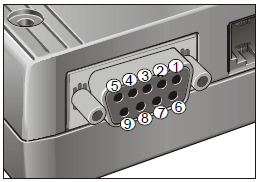
\includegraphics[scale=1]{9-pin}
\caption{9-Pin hun stik for STK-500 Spare og GSM-modem}
\end{figure}


\subsection{Drivers}
Til projektet er der blevet brugt nogle drivere fra opgaverne fra AMS-forl�bet, samt udleveret drivere til UART'en og LED'erne.
Herunder er en liste over de drivere, som vi selv har arbejdet p�.



\subsubsection{LM75}
Driveren til temperatursensoren, LM75, er baseret p� en opgave fra AMS-forl�bet.
Den kommunikerer med STK-500 vha. \IIC -bussen og kan i princippet m�le fra $-155$\degree C til $+155$\degree C, hvilket vi dog ikke har test eller finder relevant for denne opstilling.

Fra tasken \begin{code}void LM75SensorTask(void *pvParameters)\end{code} kaldes LM75-driverens funktion til, at modtage ny temperatur fra LM75-printet, vist i Listing \ref{LM75}.

\pagebreak
\begin{lstlisting}[caption=LM75's metode til at sp�rge p� ny data, style=Code-C, label=LM75]
int LM75_temperature(unsigned char SensorAddress)
{
	i2c_start();
	
	unsigned char address = ((0b01001000 | SensorAddress) << 1) | 0x01;
	i2c_write(address); //Address write
	
	unsigned char tempMSB = i2c_read(0x00); 
	unsigned char tempLSB = i2c_read(0x01);
	i2c_stop();
	
	return (tempLSB>>7) | (tempMSB<<1);
}
\end{lstlisting}

Ved at give en adressen p� slaven i \IIC -bussen som parameter, startes \IIC 'en og der sendes en foresp�rgsel p� denne slave, hvorefter denne sender sin data retur.
Eftersom temperaturen er 9 bit lang, shiftes de to l�sninger, s�ledes MSB og LSB st�r korrekt og returneres i en \begin{code}int\end{code}.





\subsubsection{LCD162}

Driveren til DragonKit, der indeholder et LCD162 display, er baseret p� en opgave fra AMS-forl�bet.
Denne kan udskrive tekst p� displayet, hvilket benyttes til at vise den aktuelle temperatur.

Der udskrives hovedsagligt \begin{code}strings\end{code} og \begin{code}ints\end{code} p� displayet. P� Listing \ref{LCDString} og Listing \ref{LCDInt} ses hvordan disse funktioner er skrevet.


\begin{lstlisting}[style=code-C++, caption=LCD162 metode til visning af en string, label=LCDString]
void LCDDispString(char* str)
{
	for(int i = 0 ; i < 32 ; i++)
	{
		if(str[i] == '\0')
			break;
		sendData(str[i]);		
	}
}
\end{lstlisting}

Listing \ref{LCDString} virker s�ledes, at den modtager en \begin{code}char*\end{code}, hvor den steppes igennem \begin{code}char\end{code} for \begin{code}char\end{code} og udskrives indtil hele strengen er udskrevet, eller har skrevet flere tegn end der kan v�re p� displayet.


\begin{lstlisting}[style=code-C++, caption=LCD162 metode til visning af en integers, label=LCDInt]
void LCDDispInteger(int i)
{
	char arr[3];
	itoa(i, arr, 10);
	LCDDispString(arr);
}
\end{lstlisting}

Listing \ref{LCDInt} virker s�ledes, at den tager imod den �nskede \begin{code}int\end{code}, som overf�res til et array med plads til 3 \begin{code}chars\end{code}\footnote{Her burde v�re 6 pladser, s� der er plads til -32768 og op til +32767}, hvorefter \begin{code}itoa\end{code}-funktionen skriver dataen in i arrayet i decimal format.
Til sidst udskrives det vha. \begin{code}LCDDispString\end{code}, vist i Listing \ref{LCDString}.


\subsection{Free RTOS}



\subsection{Ideel opbygning}

\end{document} 